% !TEX root = ../Report.tex
\subsection{DeepMedic architecture}\label{deepmedic_chapter}
DeepMedic is a 3D deep convolutional neural network architecture. It was initially designed and used for segmentations of brain lesions from 3D magnetic resonance imaging (MRI) scans. In this project this algorithm was adapted to be applied for lung and bronchus segmentations from clinical CT scans. \newline
\begin{figure}[h!]
	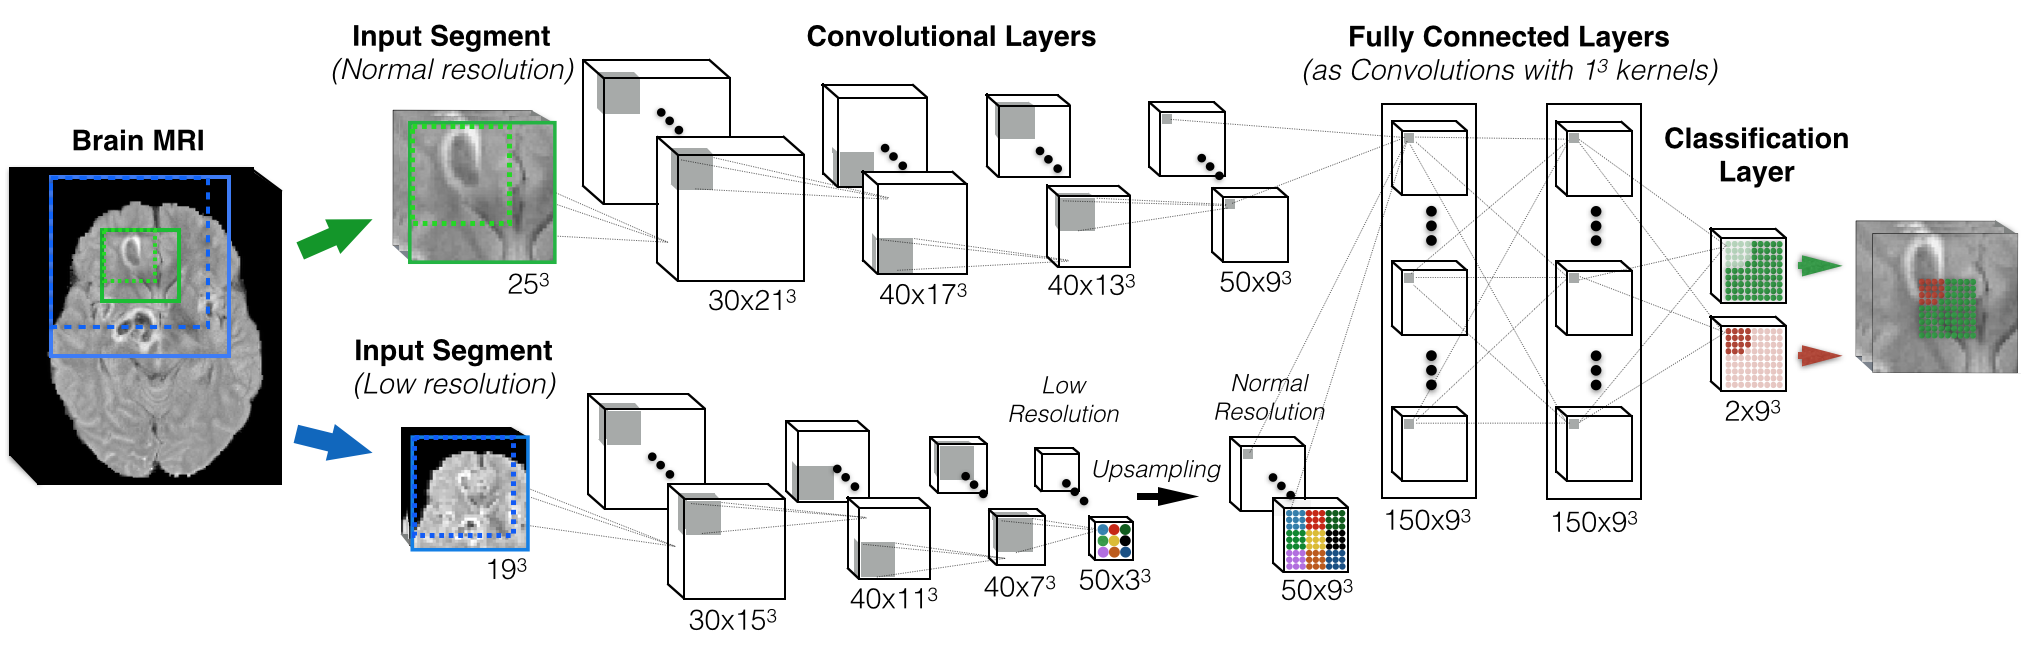
\includegraphics[width=0.49\textwidth, angle=0]{files/deepMedic.png}
	\caption{Structure of DeepMedic architecture}
	\label{deepmedic}
\end{figure}
 
A trained DeepMedic model works by detecting particular patterns and features in images. This is achieved by multi-layer convolution in the network. There are two major components in the model architecture. First there is a two path three-dimension deep convolutional neural network model used for dense segmentation (figure \ref{deepmedic} left part), followed by a three-dimension fully connected conditional random field (CRF) model which performs post-processing and handles the final hard segmentation (right part in figure \ref{deepmedic}). The double-path portion of the CNN is composed of a regular-resolution and a low-resolution path. While the regular-resolution path acts comparably to other CNN in detecting features of the images, the low-resolution pathway works to recognize lower detail features of the images which improves generalization of the final model and helps mitigate overfitting.
Each layer of the CNN model contains channels called feature maps, i.e. a group of neurons identifying a feature in the previous layer. Then features are defined by associated kernel weights. Number of inputs, outputs, feature-maps and kernels are tunable.

\subsection{U-Net architecture}
The U-Net architecture is another CNN used for image segmentation. In figure \ref{unetstructure} the structure of the U-Net is shown.\newline
\begin{figure}[h!]
	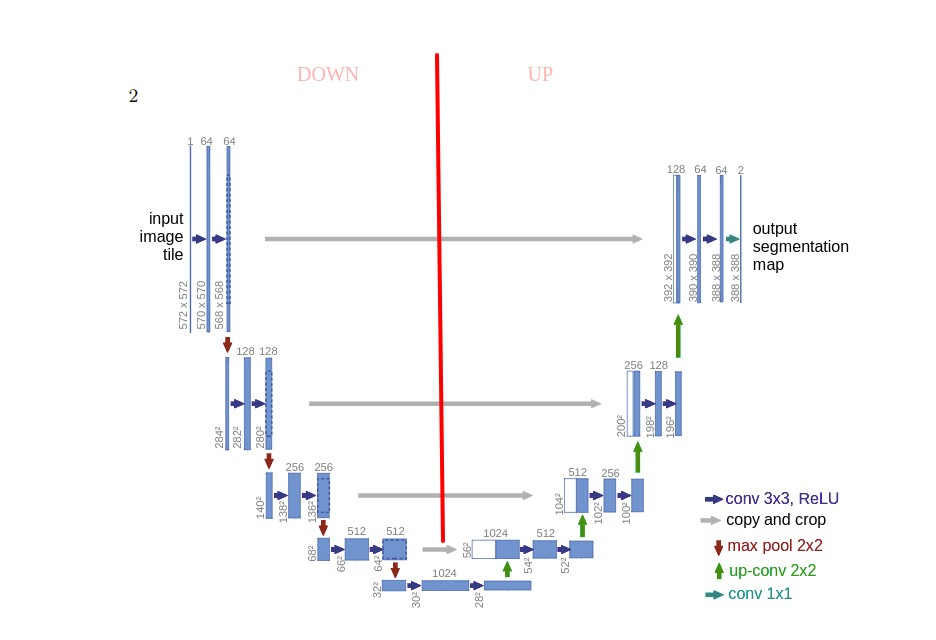
\includegraphics[width=0.49\textwidth, angle=0]{files/unetstructure.jpg}
	\caption{Structure of U-Net architecture}
	\label{unetstructure}
\end{figure}

Each blue box corresponds to a multi-channel feature map. The number of channels is denoted on top of the box. X-Y-size is provided at the lower left edge. White boxes represent copied feature maps. Arrows denote the different operations.\newline
First part is called the down or encoder part. Convolutional blocks followed by maxpool downsampling layers are applied to encode the input image into feature representations at multiple different levels. The second part of the network consists of upsampling and concatenation layers followed by regular convolution operations. The dimensions from left are expanded to meet the original image size. The grey and green arrows indicate where to concatenate feature maps together.\newline
In comparison to other fully convolutional segmentation networks, the main feature of U-Net is that while upsampling and going deeper in the networks, it also concatenates the higher resolution features from the down sampling part with upsampled features in order to better localize and learn representation.\newline
%As upsampling is sparse we need to be good prior from beginning stages to get the better localization representation. In order to get consistent size, we applied padded convolutions to keep dimensions across concatenation. Localization is one of the most important features in case of biomedical image processing. In order to localize, high resolution from the contracting path are combined with upsampled output. By this the successive convolution layer can then learn to assemble a more precise output. The main modification in our architecture was that in the upsampling part we have a large number of feature channels, which allows the network to propogate context information to high resolution layers. To predict the pixels in the border region of the image, the missing context is extrapolated by mirroring the input image.

\subsection{Metrics}\label{metrics_chapter}

\subsubsection{Dice Loss}
The models were trained by minimizing a loss function. The chosen loss function was a combination of the Dice loss coefficient and binary cross entropy. In the following equation, smoothing is added and stands for backpropagation. The Dice loss function is defined by:

\begin{equation}
dice loss = 1 - \frac{2*(Y_{true} \bigcap Y_{prediction}) + 1}{|Y_{true}| + |Y_{prediction}| + 1}
\end{equation} 

\subsubsection{BCE Dice Loss}
The other portion of the loss function used for training was binary cross-entropy (BCE) to measure the performance of the classification model. For labels y and predicted probabilities p, binary cros-entropy is:

\begin{equation}
BCE = - \frac{1}{n} \sum_{i=1}^{n}(y_i \log{(p_i)} + (1-y_i)\log{(1-p_i)})
\end{equation} 

Therefore, the BCE Dice Loss is:

\begin{equation}
Loss =  dice loss + BCE
\end{equation}

\subsubsection{Hausdorff distance}
The Hausdorff distance is a metric used to calculate the maximum distance between two corresponding segmentations.\newline
For the set of coordinates $A$ and $B$ it is defined as:

\begin{equation}
	d_{hausdorff} (A,B) = \max_{a \in A} (\min_{b \in B} d(a,b))
\end{equation} 

where $d(a,b)$ represents the Euclidean distance between the two coordinates $a$ and $b$. It can be interpreted as the maximum distance of set $B$ to set $A$ and is therefore a important metric for evaluating the difference between two label maps.

\subsubsection{Mean distance}
The mean distance is similar to the Hausdorff metric but is a measurement for the mean of the difference between two sets of coordinates.\newline
It is defined as following:

\begin{equation}
	d_{mean} (A,B) = \frac{1}{|A|} \sum_{a \in A} \min_{b \in B} d(a,b)
\end{equation}

where again $d(a,b)$ represents the Euclidean distance between the two coordinates $a$ and $b$. It can be seen as the average distance between the two sets and was used for evaluation.
